\usepackage{xcolor}
\usepackage{afterpage}
\usepackage{pifont,mdframed}
\usepackage[bottom]{footmisc}

\makeatletter
\gdef\this@inputfilename{input.txt}
\gdef\this@outputfilename{output.txt}
\makeatother

\newcommand{\inputfile}{\texttt{input.txt}}
\newcommand{\outputfile}{\texttt{output.txt}}

\newenvironment{warning}
  {\par\begin{mdframed}[linewidth=2pt,linecolor=gray]%
    \begin{list}{}{\leftmargin=1cm
                   \labelwidth=\leftmargin}\item[\Large\ding{43}]}
  {\end{list}\end{mdframed}\par}

The forty-second edition of the annual robotic ant contest is about to begin. This year, Giorgio is in charge of choosing the test that the participating robots will need to pass in order to win.

The previous organizers caused quite a mess last time (who could ever forget the \emph{Anteater arena}?), for this reason Giorgio decided to go with something easier: he will set up a grid in the guise of a labyrinth (the \emph{Labygrid}) and he will reward the ant that will traverse it in the most efficient manner.

A labygrid is nothing more than a pavement formed by $N \times M$ square-shaped tiles. For example, a valid labygrid having $N=4$ and $M=6$ can be seen in the following picture:

\begin{center}
  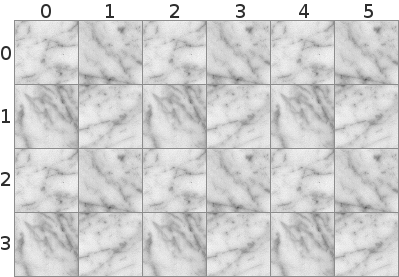
\includegraphics[width=0.8\textwidth]{floor.png}
\end{center}

The goal of the robotic ants is to reach the bottom-right corner of the $(N-1, M-1)$ tile starting from the top-left corner of the $(0, 0)$ tile. The hard part is to do that by trying to step on as few tiles as possible. The winning ant is the one that will step on the least number of tiles.

\begin{warning}
  Robotic ants can move from a tile to another by the sides or the corners. So, an ant can move to $8$ tiles at most (starting from the same tile).
\end{warning}

To spice up the game, Giorgio bought an insecticide sprayer (a special kind, for robotic ants) e he's considering whether to use it or not. Keep in mind that a robotic ant cannot step on the insecticide.

If Giorgio will feel cheerful on the day of the contest, then the insecticide will not be sprayed. However, if Giorgio will feel upset, then he will choose one or more tiles and he will start poisoning them by following this technique: he starts by spraying the poisong towards the middle of the tile and, after that, he continues to spray by moving in one of the $4$ directions: up, right, down, left.

So, if Giorgio feels especially upset, the ``trace'' left by the insecticide could reach a point where it resembles a { \Large \color{magenta} \textbf{+} } symbol on the tile. For example, in the following labygrid there are two tiles at $(0, 2)$ and at $(2, 1)$ that are really full of insecticide!

\begin{center}
  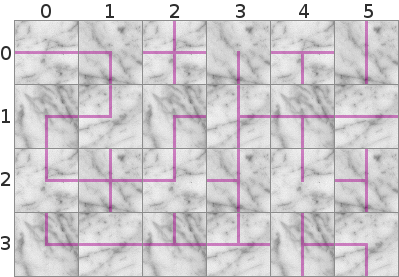
\includegraphics[width=0.8\textwidth]{floor-poison.png}
\end{center}

To help the contestants understand where the poison is located, Giorgio defines the ``poisonous factor'' for each tile. At the start, this factor is equal to $0$ for all tiles. During the application of the insecticide the factor gets increased as described by this table:

\begin{itemize} %[noitemsep,nolistsep]
  \item Spray towards the \emph{up} direction: the poisonous factor of the tile increases by $1$;
  \item Spray towards the \emph{right} direction: the poisonous factor of the tile increases by $2$;
  \item Spray towards the \emph{down} direction: the poisonous factor of the tile increases by $4$;
  \item Spray towards the \emph{left} direction: the poisonous factor of the tile increases by $8$.
\end{itemize}

\textbf{Nota:} this value does not indicate \emph{how much} a tile is poisonous, but \emph{where} it's poisonous.

\begin{warning}
  In other words, the poisonous factor is a $4$-bit binary number. If the high order bit is $1$, then the insetticide was sprayed towards the up direction; if the second bit is $1$, then the insecticide was sprayed towards the right direction; and so on.
\end{warning}

Help Giorgio to organize the upcoming edition of the robotic ant contest! Write a program to determine whether a given labygrid can be solved by a robotic ant and, if that's the case, compute the \emph{minimum number of tiles} that it will need to step on in order to do that.

\textbf{Nota:} if an ant steps multiple times on the same tile, it will be counted every time!

\Implementation
You shall submit exactly one file having extension \texttt{.c}, \texttt{.cpp} o \texttt{.pas}.

\begin{warning}
Among the attachments of this task you will find a template (\texttt{labigriglia.c}, \texttt{labigriglia.cpp}, \texttt{labigriglia.pas}) with a sample incomplete implementation.
\end{warning}

If you use the template, you'll need to implement the following function:
\begin{center}\begin{tabularx}{\textwidth}{|c|X|}
\hline
C/C++  & \verb|int cammina(int N, int M, int griglia[][MAXN]);|\\
\hline
Pascal & \begin{tabular}[x]{@{}@{}}\verb|type matrix = array of array of longint;|\\ \verb|function cammina(N, M: longint; var griglia: matrix): longint;|\end{tabular}\\
\hline
\end{tabularx}\end{center}
Where:
\begin{itemize}[nolistsep]
  \item The $N$ and $M$ integers identify the number of rows and columns of the labygrid, respectively.
  \item The \texttt{griglia} matrix, indexed from $0$ to $N-1$ for the rows and from $0$ to $M-1$ for the columns, describes the labygrid. Specifically, \texttt{griglia[i][j]} is the poisonous factor of the $(i, j)$ tile.
  \item The function must return the minimum number of tiles that a robotic ant must step on in order to solve the labygrid, or the $-1$ integer, if the labygrid is not solvable.
\end{itemize}

\InputFile
File \inputfile{} consists of $N+1$ lines.The first line has two integers $N$ and $K$ separated by a space. The next $N$ lines have $M$ integers each, and they describe the \texttt{griglia} matrix.

\OutputFile
File \outputfile{} consists of a single line, containing the $-1$ integer if a solution does not exist, or a positive integer: the answer to this task.

% Assunzioni
\Constraints
\begin{itemize}[nolistsep, itemsep=2mm]
	\item $1 \le N, M \le 1000$.
	\item $0 \le$ \texttt{griglia[i][j]} $\le 15$ for each $i, j$.
\end{itemize}

\Scoring
Your program will be tested against several test cases grouped in subtasks.
In order to obtain a subtask's score, your program needs to correctly solve all of its test cases.

\begin{itemize}[nolistsep,itemsep=2mm]
  \item \textbf{\makebox[2cm][l]{Subtask 1} [10 punti]}: Sample test cases.
  \item \textbf{\makebox[2cm][l]{Subtask 2} [10 punti]}: \texttt{griglia[i][j]} $=0$ for each $i, j$. No poison!
  \item \textbf{\makebox[2cm][l]{Subtask 3} [35 punti]}: $\min(N, M) = 1$. We should call this a \emph{labycorridor}.
  \item \textbf{\makebox[2cm][l]{Subtask 4} [20 punti]}: $N, M \le 10$.
  \item \textbf{\makebox[2cm][l]{Subtask 5} [25 punti]}: No limits.
\end{itemize}

% Esempi


\Examples
\begin{example}
\exmpfile{labigriglia.input0.txt}{labigriglia.output0.txt}%
\exmpfile{labigriglia.input1.txt}{labigriglia.output1.txt}%
\end{example}


\Explanation
The \textbf{first sample test case} is described by the second picture in the task description. A path that steps on $14$ tiles in this labygrid is the following:

\begin{center}
  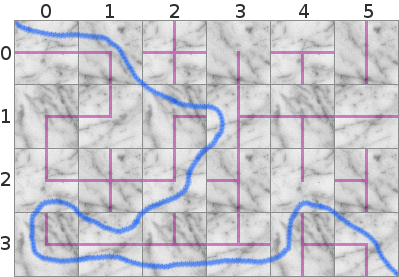
\includegraphics[width=0.8\textwidth]{floor-poison-path.png}
\end{center}
